%Summer Paper  summer-paper.tex
\documentclass[12pt]{article}
\usepackage{amssymb,latexsym}
\usepackage[round,sort]{natbib}
\usepackage{multirow,array}
\usepackage{fancyhdr}
\usepackage{lastpage}
\usepackage{graphicx}
\usepackage[bottom]{footmisc}
\graphicspath{ {summer-paper-images/} }
\usepackage[T1]{fontenc}
\usepackage{mathptmx}
\usepackage{tabu}
\usepackage{textcomp}
\usepackage{stata}
\usepackage{listings}
\newenvironment{hypothesis}{
  	\itshape
  	\leftskip=\parindent \rightskip=\parindent
  	\noindent\ignorespaces}
	
\pagestyle{fancy}
\fancyhf{}
\lhead{Knowledge Flows in Emerging Innovation Regions}
\rfoot{Page \thepage  \ of \pageref{LastPage}}
\rhead{Iyenggar}

\begin{document}
\title{Knowledge Flows in Emerging Innovation Regions:\\  Evidence from US Patent Data}
\author{Ashwin Iyenggar  (1521001) \\ ashwin.iyenggar15@iimb.ernet.in} 


\maketitle
\thispagestyle{empty}

\begin{abstract}
This article presents the findings of an exploratory analysis of the nature of knowledge flows from four emerging innovation regions as evidenced by citations of US Patents granted to inventors from these regions. Flows are mapped along two dimensions, geography (local or non-local), and citing assignee (same as that of the cited patent, or different). We find that the while the Bangalore, Beijing, Israel and Austin regions all show a much higher share of knowledge flow to the rest of the world than to within the region, the Bangalore region's local knowledge flows have been practically non-existent.
\end{abstract}


{Keywords:} Innovation Regions, Clusters, Knowledge Flows

\section{Introduction}\label{S:Introduction}
Literature in the strategy area has highlighted the importance of innovation as a source of competitive advantage in firms. Scholars have highlighted that firms have tended to adopt two distinct strategies in seeking to capture greater advantages in knowledge flows: a) geographic clustering \citep{Porter2003}, and b) the globalization of R\&D \citep{Almeida1996}. Scholars have in the past conclusively demonstrated that the bay area in California (that includes the city of San Francisco and is hereafter referred to as Silicon Valley for convenience) demonstrates strong  cluster characteristics in that there are strong flows of knowledge within and across firms from within the same geographical area (Citation needed). While the benefits to such geographical localization of knowledge flows \citep{Porter2003} has been celebrated as an important aspect of the superior economic performance of Silicon Valley, there has been little work that has explored the same for  emerging innovation regions of Bangalore, Beijing, Israel and Austin. In this article, we analyze the nature of knowledge flows at the level of the region in aggregate rather than focus on specific industries of technologies as have been done in past studies \citep{Lecocq2016}.  In order to understand if these emerging innovation regions are trending toward clustering \citep{Jaffe1993} or globalization or knowledge flows or both, we categorize all knowledge flows along two dimensions: a) as a relationship between the location of the creator of the knowledge and the location of the user of the knowledge, and b) as a relationship between the owner of the knowledge and the beneficiary of the knowledge. This classification allows us to see knowledge flows in four non-intersecting categories as illustrated in Table ~\ref{table:matrix}

\begin{table}
\begin{centering}
\label{table:matrix}
\begin{tabular}{c|c|c|c|}
\multicolumn{1}{c}{}&\multicolumn{1}{c}{}&\multicolumn{2}{c}{Location}\\
\cline{2-4}
&&{Same}&Different\\
\cline{2-4}
\multirow{2}*{Firm}&{\rotatebox{90}{Same}}&{\hfill Independent Research Centre}&{\hfill Geographic Diversification}\\
\cline{2-4}
&{\rotatebox{90}{Different}}&{Cluster}&{Diffusion}\\\cline{2-4}
\end{tabular}
\caption {Categories of Knowledge Flows}
\end{centering}
\end{table}

In Table ~\ref{table:matrix}, the quadrants on the left column indicate knowledge flows within the region whereas the quadrants in the right column indicate knowledge flows to other regions. We are  interested in understanding if the emerging innovation clusters of Bangalore, Beijing, Israel, and Austin show the characteristics of  geographical clustering \citep{Jaffe1993}. We use the Boston region and Silicon Valley as  leading innovation clusters to inform our reference point in studying the emerging innovation clusters.

\section{Research Design}
We use the United States patents data as made available on PatentsView.org as our primary data source to empirically investigate knowledge flow from the four emerging innovation regions identified for this study. Based on our 2x2 framework depicted in Table ~\ref{table:matrix}, we examine two primary relationships taken together: first, the relationship between the location of the citing patent's assignee and that of the cited patent's inventor, and second, the relationship between the identity of the citing patent's assignee and the identity of the citing patent's assignee. When the location of the cited patent's inventor is the same as the location of the citing patent's assignee, and the cited patent's assignee is the same as the citing patent's assignee, we classify the flow of knowledge in the top left quadrant, and label that an Independent Research Centre. When the locations of the cited inventor and the citing assignee are different, but the  identity of the assignee on the cited and citing patents are identical, we classify the flow of knowledge into the top right quadrant and label that Geographic Diversification. When the former dimensions match, but the latter dimensions do not, the knowledge flow is classified into the lower left quadrant and labelled Cluster. Finally when both dimensions do not match, we place that knowledge flow into the bottom right quadrant and label it Diffusion.

There seem to be two ways to position time in studies of knowledge flow. The first is to assign the grant date of the citing patent to the knowledge flow between the citing patent and the cited patent. While this measure captures the time when existing knowledge is utilized to build new knowledge, this approach suffers from the problem of the time lag between the patenting of the original knowledge and the patenting  of the new knowledge. When captured in this form, knowledge flows are often seen to be falling off a cliff in the later years of the sample. The second method is to assign the grant date of the cited patent to the knowledge flow. This resolves the problem of the data seeming to fall off a cliff toward the later years, but ascribes value to actions of the past. While this measure may help understand which periods generated highly valuable knowledge, it would be less useful in understanding the trend into the present. Our view is that both approaches have their own merit and that it may be useful to construct out model based on both. However, in this exploratory study, we focus on the former, and therefore the rapid descent in knowledge flows in the years leading to 2016 should be understood as reflecting the lagged effect of patent citations. On the flip side though this view of the data gives readers an accurate view of the level of flows that actually occurred during any past period.

The current study is an exploratory study to identify the nature of knowledge flows in the regions selected. While do not endeavor to hypothesize the implications of such knowledge flows in this study, we do expect to lay the ground work with data collection, data organization and preliminary analysis so as to build specific testable hypotheses in future extensions. We therefore conclude our current study with an analysis of region wise knowledge flows rather than delve into industry specific flows, though that would an interesting study to conduct on its own.

\begin{figure}[h]
\begin{centering}
  \includegraphics[scale=0.2]{PatentLocations}
  \caption{US Patent Inventor Locations 1976-2016}
  \label{fig:patentlocations}
\end{centering}
\end{figure}

\section{Data and Methods}
We utilize the patents database as available on PatentsView.org for the entire period for which the data is available (1976 onwards).  Table ~\ref{table:aggregate} provides some statistics that describe the size of the data set. As has been the norm in prior literature, the United States Patents Data has been accepted as a good approximation for the inventive knowledge generated globally. Figure ~\ref{fig:patentlocations} provides a pictorial view of the various locations that inventors and assignees have patented from over the period from 1976-2015. While geographic coverage is by itself not indicative of completeness (it maybe that only a few of the patentable inventions in foreign locations may be patented in the United States), the extent of the geographical coverage must make it clear that the United States is indeed the patenting region of choice. We therefore choose to rely on data from the PatentsView database to base our empirical analysis on knowledge flows from each of the four regions identified.

\begin{table}
\begin{centering}
\label{table:aggregate}
\begin{tabular}{|c|c|}
\hline
Statistic&Value\\
\hline
Count of Knowledge Flows 1976-2015&80,728,767\\ \hline
Unique Patents 1976-2015&5,915,850\\ \hline
Unique Inventors 1976-2015&3,287,306\\ \hline
Unique Locations 1975-2015&128,911\\ \hline
Patents Without Assignee 1976-2015&39,302\\ \hline
\end{tabular}
\caption {Aggregate Statistics of PatentsView Data 1976-2015}
\end{centering}
\end{table}

Our first task was to define the extent of the regions themselves. While the patents data comes with city, state and country information, this information was found to be incomplete and not completely reliable. We therefore used Geographical Information Systems (GIS or Mapping) software and publicly available shapefiles for each of the administrative units. We then defined each of the regions of interest as a collection of neighboring administrative units. Zoomed out, this has been depicted in Figure ~\ref{fig:AsianClusters} and Figure \ref{fig:USClusters}. A zoomed in, detailed view of these regions can be made available on request. It is to be noted that the selection of the regions as defined here was based on an assessment of a reasonable geographic boundary based on existing administrative boundaries (taluks in India, counties in the US etc). There maybe a case to review this and define these regions as per an accepted norm. As things stand, our implementation is able to take any structure of a geographical boundary and analyze the flows of knowledge from that.

We used the regions shapefiles generated to select the patent inventor and assignee locations for each of the regions of interest. Since it is possible for a single inventor to have been located at different locations for each of his/her patents, and similarly for an assignee (though less likely), we take care to assign location at the level of each flow of knowledge. A single citation with several inventors would therefore include multiple inventor-location to cited-patent assignee-location relationships. To ensure that none of the locations within the regions of interest are missed, we perform a visual geographic test to ensure that none of the patenting locations being excluded as being outside the scope of the inventor locations of interest in this study are within any of our defined regions. Figures ~\ref{fig:BangalorePrime}, ~\ref{fig:BeijingPrime}, ~\ref{fig:IsraelPrime}, and ~\ref{fig:AustinPrime} are pictorial snapshots of these verifications.

We use the uspatentcitation.tsv data file as the primary source of information regarding all patent citations for the period 1976-2015. We derive fine grained inventor data from rawinventor.tsv and fine grained assignee data from rawassignee.tsv. Each assignee and each inventor is assigned a unique rawlocation\_id for each patent they have been connected with. We use this information from rawlocation.tsv to therefore map locations not just to inventors and assignees, but to inventor-for-a-specific-patent and assignee-for-a-specific-patent. This allows us to capture changes in location of both inventors and assignees. While we have not looked at the question of mobility of inventors, or that of assignees, our approach to capturing the data allows us to extend along this dimension. Finally we obtained detailed patent and assignee information from patent.tsv and assignee.tsv. A STATA do file for the merge of data for the Bangalore cluster has been provided in the Code section of the appendix. 

Our approach was to not drop or delete any piece of data during our analysis. However, there was one unavoidable decision relating to some patents not having assignees. We had to drop a total of 39,302 patents that had no assignee.\footnote{We reached out to the person managing the PatentsView.org database with this query. Here is his response on the topic, verbatim: "We parse patent data from official USPTO files. If there is no assignee - it means there is no such data in those files. The reason why you see assignees on the patents you attached is because Google (and some other companies) automatically assign such patents to the inventor (e.g. 3930331 is invented by Janet A. Simeone and assigned to her too while this is not entirely accurate from the data perspective). The other thing is that there is a notion of post-grant assignee - i.e. if the inventor transfers (sells) the rights to a patent to a different assignee at a later phase. Information on these post-grant assignees is not easily available and have to be parsed from other data sources. We hope to include this information into PatentsView at a future stage."}

\section{Results}
Table ~\ref{table:regions} provides some key statistics on the comparison across the four regions we studied, and the two larger innovation regions of the greater Boston area, and of Silicon Valley. We note that Bangalore and Beijing are somewhat comparable when it comes to the number of patents and to the number of inventors in the region but there is a noticeable gap in the number of patent citations received. At 258,438 patent citations, Israel is significantly ahead of both Beijing and Bangalore in aggregate terms. It is interesting to note, however that on an aggregate level, Israel seems to be doing better than Austin.


\begin{table}
\begin{centering}
\label{table:regions}
\begin{tabular}{|c|c|c|c|c|c|c|}
\hline
Statistic&BLR&BEI&ISR&AUS&BOS&SIV\\ \hline
Unique Patents 1976-2015&8,947&11,883&40,818&21,082&121,592&374,223 \\ \hline
Unique Inventors 1976-2015&7,315&9,106&25,972&5,747&52,627&141,048\\ \hline
Citations 1976-2015&23,937&30,025&258,439&165,562&829,451&1,472,575\\ \hline
\end{tabular}
\caption {Statistics of PatentsView Data by Region 1976-2015}
\end{centering}
\end{table}

We provide our results for each of the four regions along the 2x2 framework developed earlier in the article. 
\subsection{Bangalore}

\begin{figure}[h]
\begin{centering}
  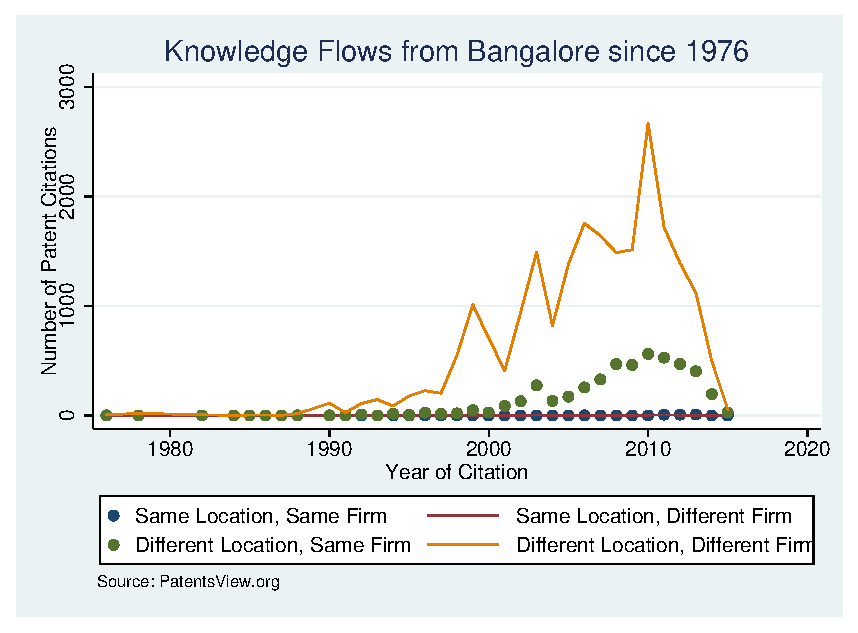
\includegraphics[width=\textwidth]{Bangalore1976}
  \caption{Knowledge Flows from Bangalore}
  \label{fig:Bangalore1976}
\end{centering}
\end{figure}

Figure \ref{fig:Bangalore1976} depicts the extent of knowledge flows from patents co-invented by at least one inventor resident in Bangalore at the time of the invention. We note that there has been a trend of rising knowledge flows since 1990. We specifically note that the number of citations from other regions has been consistently higher than those from within the region. This is hardly surprising since I would expect a wider adoption of the knowledge among the rest of world just by virtue of the relative sizes of the region of interest as compared to that of the rest of the world. This is borne out in each of the four regions as Figure \ref{fig:Beijing1976} depicts for Beijing, Figure \ref{fig:Israel1976} depicts for Israel, and Figure \ref{fig:Austin1976} depicts for Austin. However what is unexpected here is that the number of local knowledge flows seem to be stuck close to zero. This is clearer in Figure \ref{fig:BangaloreLocal1976} where we only consider the local flows of knowledge. As is clear from the figure, the number of citations to locally generated knowledge is not just a very low value in absolute terms, but that the number has just not picked up over the years.

\begin{figure}[h]
\begin{centering}
  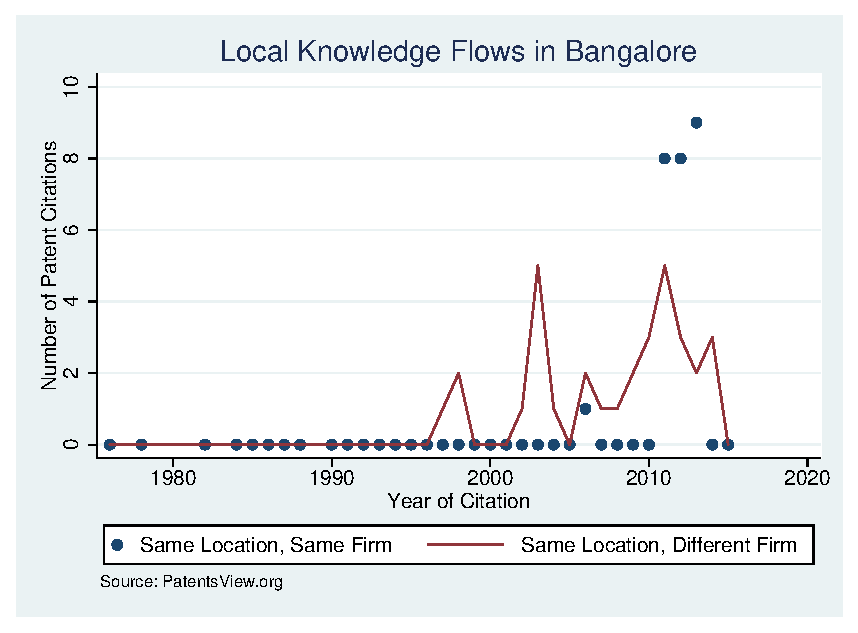
\includegraphics[width=\textwidth]{BangaloreLocal1976}
  \caption{Local Knowledge Flows in Bangalore}
  \label{fig:BangaloreLocal1976}
\end{centering}
\end{figure}


\subsection{Beijing}

\begin{figure}[h]
\begin{centering}
  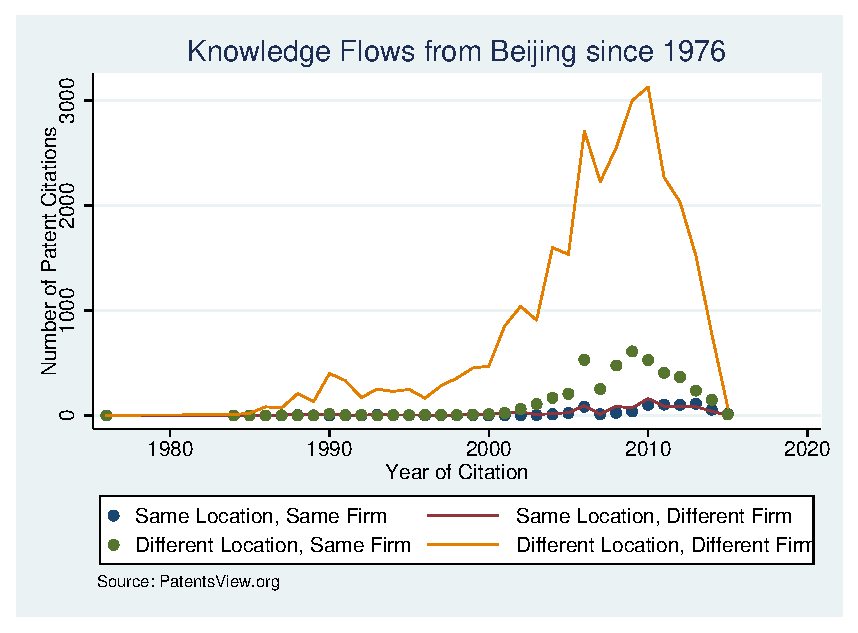
\includegraphics[width=\textwidth]{Beijing1976}
  \caption{Knowledge Flows from Beijing}
   \label{fig:Beijing1976}
\end{centering}
\end{figure}


Figure \ref{fig:Beijing1976} depicts the extent of knowledge flows from patents co-invented by at least one inventor resident in Beijing at the time of the invention. We note that there has been a trend of rising knowledge flows since the mid 1980\textquotesingle\ s. As in Bangalore, we note that the number of citations from other regions has been consistently higher than those from within the region. Chinese inventions have therefore witnessed  a wider adoption of the knowledge amongst the rest of world. Figure \ref{fig:BeijingLocal1976} zooms into the local flows of knowledge for Beijing. We note here that the number of citations are on the increase, and that the number of flows to same firms and to different firms are up in step. 

\begin{figure}[h]
\begin{centering}
  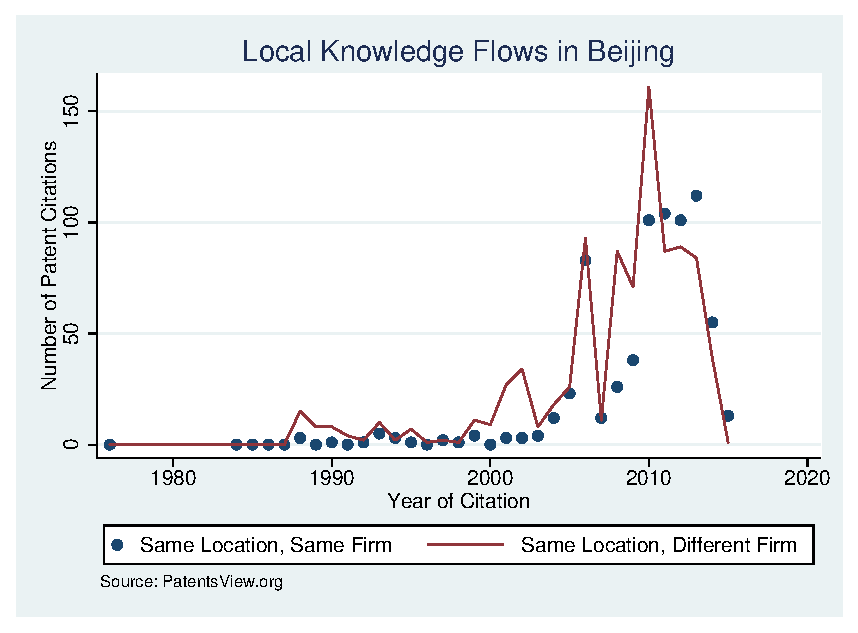
\includegraphics[width=\textwidth]{BeijingLocal1976}
  \caption{Local Knowledge Flows in Beijing}
   \label{fig:BeijingLocal1976}
\end{centering}
\end{figure}



\subsection{Israel}

\begin{figure}[h]
\begin{centering}
  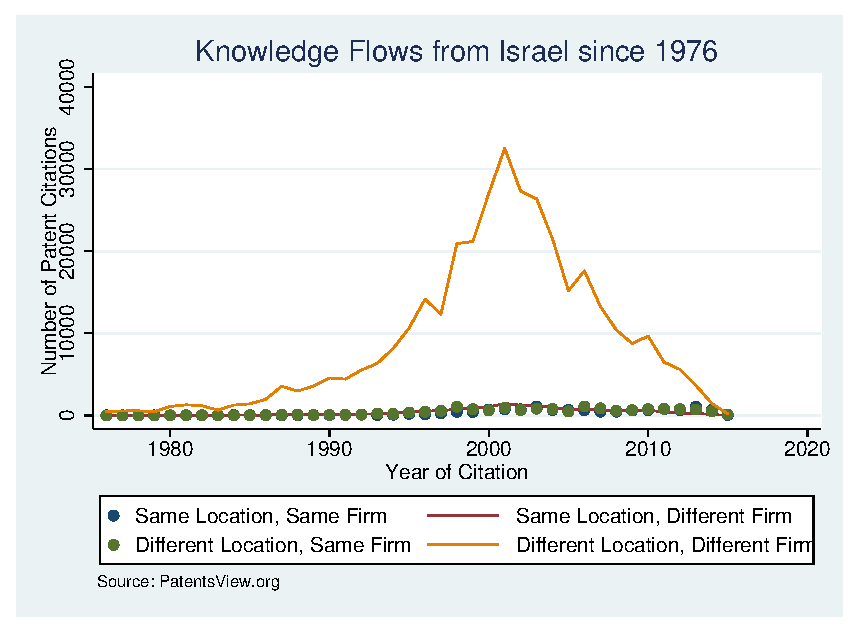
\includegraphics[width=\textwidth]{Israel1976}
  \caption{Knowledge Flows from Israel}
  \label{fig:Israel1976}
\end{centering}
\end{figure}
Figure \ref{fig:Israel1976} depicts the extent of knowledge flows from patents co-invented by at least one inventor resident in Israel at the time of the invention. We notice here a peculiar characteristic, where one of the four quadrants (Diffusion quadrant) dramatically dominates. Also suprising is the steep rise and fall in the number of such flows around the year 2000. The most noticeable feature about Israel however, is the sheet numbers. While with Bangalore had a few handful to a few tens of flows, and Beijing had a few hundreds, Israel's flows go into the tens of thousands. Figure \ref{fig:IsraelLocal1976} clarifies that the local flows of knowledge are also extremely strong, and that like Beijing flows to same firms and different firms are both growing and are in step. 

\begin{figure}[h]
\begin{centering}
  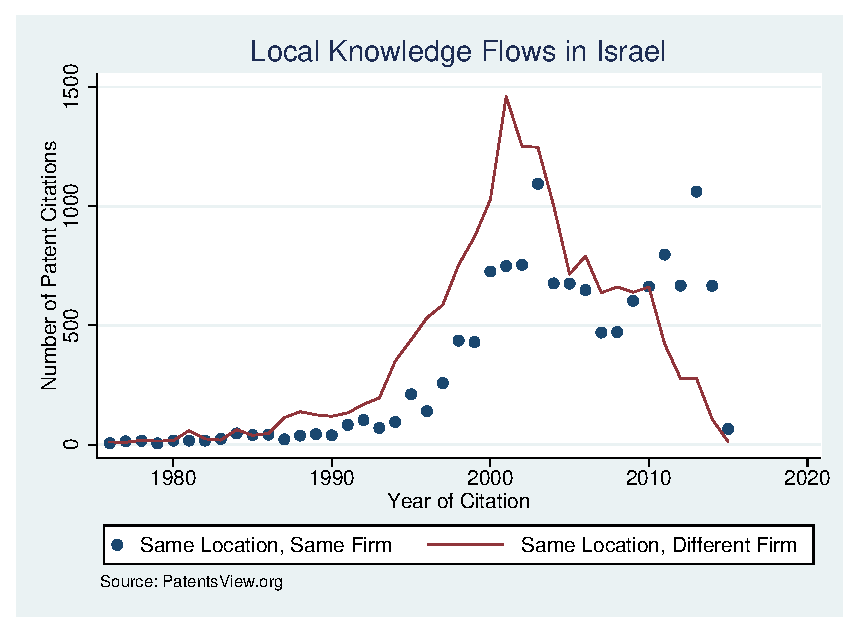
\includegraphics[width=\textwidth]{IsraelLocal1976}
  \caption{Local Knowledge Flows in Israel}
  \label{fig:IsraelLocal1976}
\end{centering}
\end{figure}

\subsection{Austin}

\begin{figure}[h]
\begin{centering}
  \includegraphics[width=\textwidth]{Austin1976}
  \caption{Knowledge Flows from Austin}
  \label{fig:Austin1976}
\end{centering}
\end{figure}

Figure \ref{fig:Austin1976} depicts the extent of knowledge flows from patents co-invented by at least one inventor resident in Austin at the time of the invention. Similar to Israel, there seems to have been a rapid rise and then a rapid fall in the quantum of knowledge flows in the late 1990\textquotesingle\ s. Figure \ref{fig:AustinLocal1976} demonstrates that local flows of knowledge have been steady, and that both the lines seem to have been moving in step.

\begin{figure}[h]
\begin{centering}
  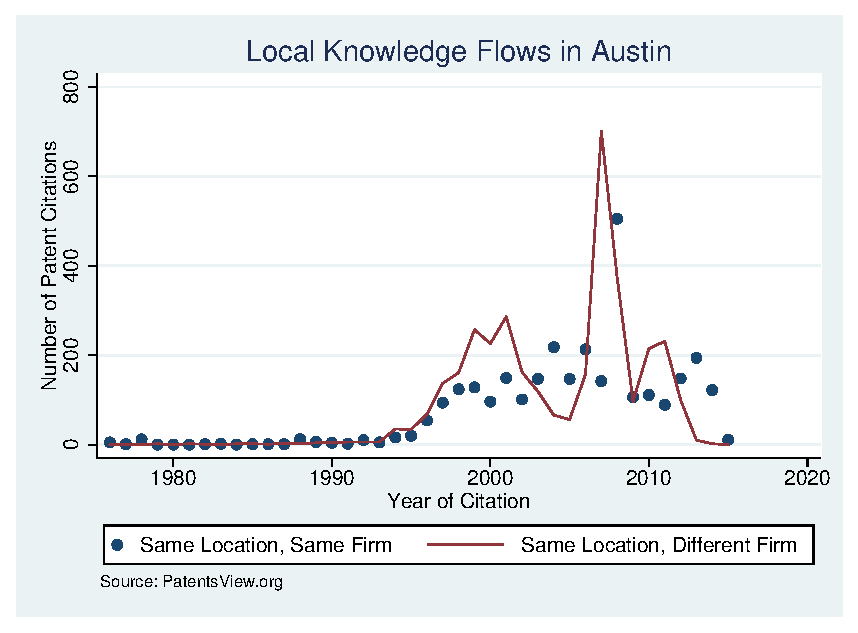
\includegraphics[width=\textwidth]{AustinLocal1976}
  \caption{Local Knowledge Flows in Austin}
  \label{fig:AustinlLocal1976}
\end{centering}
\end{figure}

\section{Discussion}
Our preliminary analysis of the knowledge flows throws up some very interesting results. First, the local flows in the Bangalore cluster are quite an anomaly as compared to the others. While it is not clear why this may be the case, one possible extension to the study could be to examine the nature of patents published by Bangalore inventors vis-a-vis that of other regions. Second, we note that in each of Beijing, Israel, and Austin, the local flows to the same firm and to different firms are both stable or growing and in step with each other. This indicates that the knowledge generated locally is not confined to the firm or to the parent firm, but that other local firms are building on top of the knowledge generated locally. Third, we note that Israel operates at a higher level of knowledge throughput than Austin, and may clearly need to studied more closely for lessons for Bangalore and Beijing. Finally, the rapid rise and fall in total number of knowledge flows evidenced in both Israel and Austin are interesting to investigate further. What led to the rise? Was it a particular technology?

\section{Limitations and Future Work}
An amateur study as is one performed here is likely to require a very long section on limitations and future work. However, we focus on building hypotheses with the data collected as potential next steps. From this perspective we suggest that the four interesting observations highlighted in the discussion section maybe the ones worthy of further work. Additionally, much work needs to be done in analyzing the literature and basing future work on sound a theoretical framework.


\section{Conclusion}\label{S:Conclusion}
In this elementary study of the flows of knowledge from four specific innovative regions of the world, we have tried to organize this along the two dimensions of location and ownership \footnote{I am grateful to Prof. Sai Yayavaram for having proposed this framework as being an appropriate one for analyzing patent flows. To him should go the credit for much of the ideation and structure of this project. I however, singly own the responsibility for errors and omissions}. Organizing the data in this form has allowed us to surface some interesting facts, and potentially interesting research questions. 

\bibliography{/Users/aiyenggar/OneDrive/code/bibliography/ae,/Users/aiyenggar/OneDrive/code/bibliography/fj,/Users/aiyenggar/OneDrive/code/bibliography/ko,/Users/aiyenggar/OneDrive/code/bibliography/pt,/Users/aiyenggar/OneDrive/code/bibliography/uz} 
\bibliographystyle{apalike}

\appendix

\section{Code}
\lstinputlisting{summer-paper-images/120-cgcd_BLR.do}

\section{Spatial Data}

\begin{figure}[h]
\begin{centering}
  \includegraphics[width=\textwidth]{AsianClusters}
  \caption{Geographic Definitions of Bangalore, Beijing and Israel Regions}
   \label{fig:AsianClusters}
\end{centering}
\end{figure}

\begin{figure}[h]
\begin{centering}
  \includegraphics[width=\textwidth]{USClusters}
  \caption{Geographic Definitions of Austin, Boston and Silicon Valley Regions}
   \label{fig:USClusters}
\end{centering}
\end{figure}


\begin{figure}[h]
\begin{centering}
  \includegraphics[width=\textwidth]{BangalorePrime}
  \caption{Spatial Verification of Locations Defined as Bangalore}
   \label{fig:BangalorePrime}
\end{centering}
\end{figure}

\begin{figure}[h]
\begin{centering}
  \includegraphics[width=\textwidth]{BeijingPrime}
  \caption{Spatial Verification of Locations Defined as Beijing}
   \label{fig:BeijingPrime}
\end{centering}
\end{figure}

\begin{figure}[h]
\begin{centering}
  \includegraphics[width=\textwidth]{IsraelPrime}
  \caption{Spatial Verification of Locations Defined as Israel}
   \label{fig:IsraelPrime}
\end{centering}
\end{figure}

\begin{figure}[h]
\begin{centering}
  \includegraphics[width=\textwidth]{AustinPrime}
  \caption{Spatial Verification of Locations Defined as Austin}
   \label{fig:AustinPrime}
\end{centering}
\end{figure}


\end{document}
